\documentclass[10pt]{beamer}
\usepackage[utf8]{inputenc}
\usepackage{xeCJK}
\usepackage{graphicx}
\usepackage {mathtools}
\usepackage{utopia} %font utopia imported
\usetheme{CambridgeUS}
\usecolortheme{dolphin}

% Russian language
\usepackage[russian]{babel}
\usepackage[utf8]{inputenc}
\usepackage[T2A, T1]{fontenc}
\usepackage{fontspec}
\usefonttheme{serif}
\setmainfont{Times New Roman}

% set colors
\definecolor{myNewColorA}{RGB}{126,12,110}
\definecolor{myNewColorB}{RGB}{165,85,154}
\definecolor{myNewColorC}{RGB}{203,158,197}
\setbeamercolor*{palette primary}{bg=myNewColorC}
\setbeamercolor*{palette secondary}{bg=myNewColorB, fg = white}
\setbeamercolor*{palette tertiary}{bg=myNewColorA, fg = white}
\setbeamercolor*{titlelike}{fg=myNewColorA}
\setbeamercolor*{title}{bg=myNewColorA, fg = white}
\setbeamercolor*{item}{fg=myNewColorA}
\setbeamercolor*{caption name}{fg=myNewColorA}
\usefonttheme{professionalfonts}
\usepackage{natbib}
\usepackage{hyperref}
%------------------------------------------------------------
%\titlegraphic{\includegraphics[height=1.5cm]{nku-logo.eps}}

%\setbeamerfont{title}{size=\large}
%\setbeamerfont{subtitle}{size=\small}
%\setbeamerfont{author}{size=\small}
%\setbeamerfont{date}{size=\small}
%\setbeamerfont{institute}{size=\small}
\title[One slide talk]{One slide talk}
%\subtitle{The Top Forwards in the World}
\author[Андрей Веприков]{Андрей Веприков}

%\institute[idk@rma.com]{ Nankai University

%School of Soccer}
\date[16 марта 2023]
{16 марта 2023}

%------------------------------------------------------------
%This block of commands puts the table of contents at the 
%beginning of each section and highlights the current section:
%\AtBeginSection[]
%{
%  \begin{frame}
%    \frametitle{Contents}
%    \tableofcontents[currentsection]
%  \end{frame}
%}
%\AtBeginSection[]{
%  \begin{frame}
%  \vfill
%  \centering
%  \begin{beamercolorbox}[sep=8pt,center,shadow=true,rounded=true]{title}
%    \usebeamerfont{title}\insertsectionhead\par%
%  \end{beamercolorbox}
%  \vfill
%  \end{frame}
%}
%------------------------------------------------------------

\begin{document}

%The next statement creates the title page.
%\frame{\titlepage}
%\begin{frame}
%\frametitle{Содержание}
%\tableofcontents
%\end{frame}
%------------------------------------------------------------
\section{One slide talk}
    \begin{frame}{On the problem of repeated supervised learning}
        \footnotesize
        \begin{minipage}[t]{0.44\textwidth} 
            \textbf{Немного обозначений}:
            \begin{enumerate}
                \item $\mathbf{R}$ -- множество функций распределения

                \item $\text{D}$ -- алгоритм обучения модели в результате применения которого изменяется распределение признаков.
            \end{enumerate}
            \textbf{Постановка нашей задачи:}
            $$g_{t+1} = \text{D}(g_t) ~~\forall t \in \mathbb{N}, ~g_0 \in \mathbf{R}$$

            \textbf{Вопросы, которые мы хотим изучить:}
            \begin{enumerate}
                \item При каких условиях оператор $\text{D}$ переводит $\mathbf{R}$ в $E \subseteq \mathbf{R}$

                \item При каких условиях оператор $\text{D}$ является сжимающим отображением

                \item При каких условиях оператор $\text{D}$ имеет неподвижную точку

                \item При каких условиях оператор $\text{D}$ переводит начальное распределение $f_0$ в в дельта функцию
            \end{enumerate}
        \end{minipage}
        \hfill
        \begin{minipage}[t]{0.53\textwidth} 
            \textbf{Постановка эксперимента:}
            \begin{figure}
                \centering
                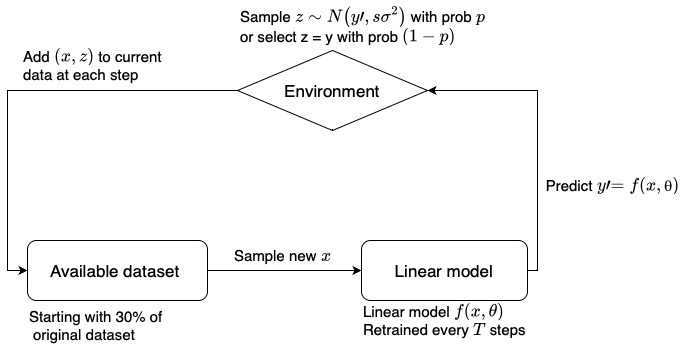
\includegraphics[scale=0.2]{pictures/Experiment_setup.png}
                \label{ex_setup}
            \end{figure}
            %Рассмотрим вектор $(\mathbf{x^i}, y_i)^T$, где $\mathbf{x^i} \in \mathbf{X}$ 
            %-- матрица объекты-признаки и $y_i \in \mathbf{y}$ -- значение целевой переменной объекта $i$.
            \textbf{Предварительные итоги эксперимента:}
            \begin{figure}
                \centering
                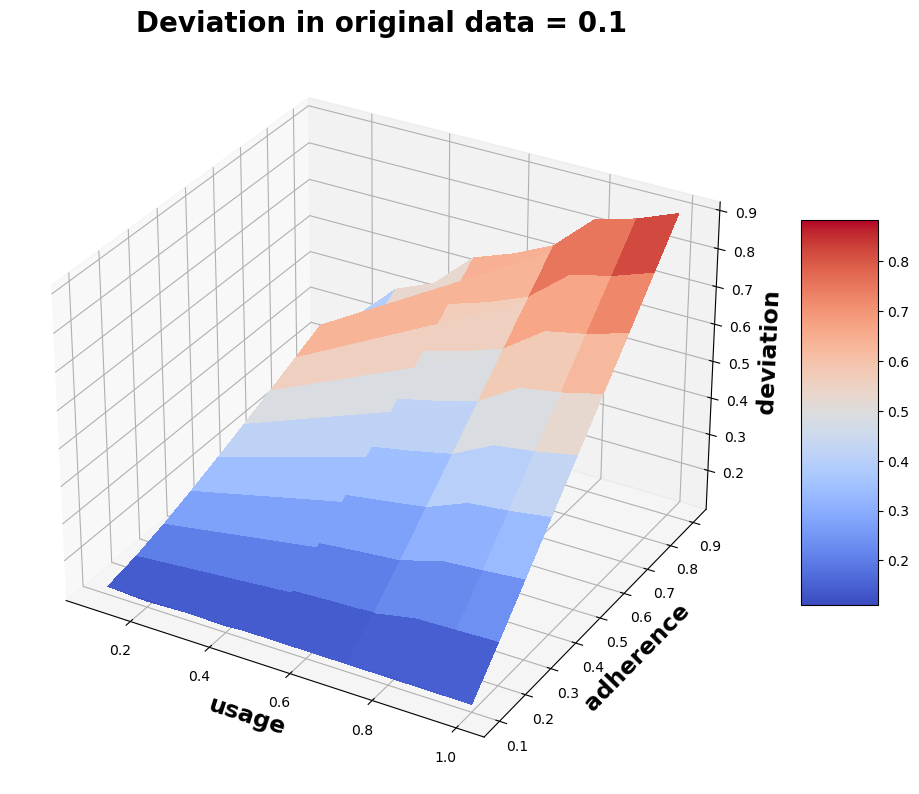
\includegraphics[scale=0.19]{pictures/3D plot.png}
                \label{res}
            \end{figure}
            %\begin{enumerate}
                %\item Линейная модель
                %\item Функции $f_t \rightarrow \delta$
                %\item Уменьшение дисперсии $\mathbf{y} - \mathbf{y_{\text{pred}}}$
            %\end{enumerate}
        \end{minipage}
    \end{frame}

\end{document}
